% !TEX program = xelatex
% 中文主稿：AISS 2026 挑战赛
% 编译：tools/build_paper.sh（xelatex ×2 + bibtex）
% 纪律：正文不手抄任何实验数字，一律引用 numbers.tex 宏；
%       批次冻结后重跑 tools/gen_paper_numbers.py 即全文更新。
\documentclass[10.5pt,twocolumn]{ctexart}
\usepackage[a4paper,top=2.2cm,bottom=2.4cm,left=1.8cm,right=1.8cm,columnsep=0.75cm]{geometry}
\usepackage{graphicx}
\usepackage{booktabs}
\usepackage{amsmath}
\usepackage[numbers,sort&compress]{natbib}
\usepackage{xcolor}
\usepackage{caption}
\usepackage{hyperref}
\hypersetup{colorlinks=true,linkcolor=black,citecolor=blue!50!black,urlcolor=blue!50!black}
\captionsetup{font=small,labelfont=bf}
\setlength{\bibsep}{2pt}
\renewcommand{\bibfont}{\small}

% 自动生成（tools/gen_paper_numbers.py），勿手改
% 生成日期 2026-09-13
\newcommand{\ValidRuns}{11}
\newcommand{\TargetRuns}{12}
\newcommand{\DraftBadge}{}
\newcommand{\DraftBadgeEn}{}
\newcommand{\IsoIvNone}{29.4}
\newcommand{\LonIvNone}{37.7}
\newcommand{\IsoPostNone}{27.2}
\newcommand{\IsoRebNone}{-2.2}
\newcommand{\NNone}{3}
\newcommand{\IsoIvCasework}{7.9}
\newcommand{\LonIvCasework}{29.4}
\newcommand{\IsoPostCasework}{27.5}
\newcommand{\IsoRebCasework}{+19.6}
\newcommand{\NCasework}{3}
\newcommand{\IsoIvTimebank}{24.7}
\newcommand{\LonIvTimebank}{36.3}
\newcommand{\IsoPostTimebank}{25.6}
\newcommand{\IsoRebTimebank}{+0.8}
\newcommand{\NTimebank}{3}
\newcommand{\IsoIvPlatform}{23.5}
\newcommand{\LonIvPlatform}{35.4}
\newcommand{\IsoPostPlatform}{27.5}
\newcommand{\IsoRebPlatform}{+4.0}
\newcommand{\NPlatform}{2}
\newcommand{\CaseworkIvReduction}{73\%}
\newcommand{\PairIvCasework}{-21.5}
\newcommand{\PairIvCaseworkN}{3}
\newcommand{\PairRebCasework}{+21.8}
\newcommand{\PairRebCaseworkN}{3}
\newcommand{\PairIvTimebank}{-4.7}
\newcommand{\PairIvTimebankN}{3}
\newcommand{\PairRebTimebank}{+3.1}
\newcommand{\PairRebTimebankN}{3}
\newcommand{\PairIvPlatform}{-5.6}
\newcommand{\PairIvPlatformN}{2}
\newcommand{\PairRebPlatform}{+4.8}
\newcommand{\PairRebPlatformN}{2}
\newcommand{\DelayCostCasework}{+0.15}
\newcommand{\DelayCostTimebank}{+0.18}
\newcommand{\DelayCostPlatform}{+0.00}
\newcommand{\TimingSeeds}{20}
\newcommand{\RulesBaselineOverall}{15.0}
\newcommand{\RulesRebCwLo}{+7.9}
\newcommand{\RulesRebCwHi}{+9.5}
\newcommand{\RulesRebTb}{+2.1}
\newcommand{\CaseCwRun}{casework\_s1}
\newcommand{\CaseCwAgent}{18}
\newcommand{\CaseCwLonWd}{0.19}
\newcommand{\CaseCwLonEnd}{0.50}
\newcommand{\CaseCwTiesWd}{7}
\newcommand{\CaseCwTiesEnd}{6}
\newcommand{\LoopIters}{5}
\newcommand{\LoopBestDesc}{casework start=4 dur=12}
\newcommand{\LoopBestScore}{7.70}
\newcommand{\FocIvNone}{56.9}
\newcommand{\FocPostNone}{51.8}
\newcommand{\RulIvNone}{17.7}
\newcommand{\RulPostNone}{16.7}
\newcommand{\FocShareNone}{58\%}
\newcommand{\FocLonIvNone}{0.56}
\newcommand{\FocLonPostNone}{0.58}
\newcommand{\RulLonIvNone}{0.30}
\newcommand{\RulLonPostNone}{0.33}
\newcommand{\FocIvCw}{13.0}
\newcommand{\FocPostCw}{63.0}
\newcommand{\RulIvCw}{5.8}
\newcommand{\RulPostCw}{12.3}
\newcommand{\FocShareCw}{49\%}
\newcommand{\FocLonIvCw}{0.42}
\newcommand{\FocLonPostCw}{0.52}
\newcommand{\RulLonIvCw}{0.24}
\newcommand{\RulLonPostCw}{0.29}
\newcommand{\PFocIvCw}{-44.0}
\newcommand{\PFocRebCw}{+55.1}
\newcommand{\PRulIvCw}{-11.9}
\newcommand{\PRulRebCw}{+7.5}
\newcommand{\FocIvTb}{45.8}
\newcommand{\FocPostTb}{52.8}
\newcommand{\RulIvTb}{15.7}
\newcommand{\RulPostTb}{13.9}
\newcommand{\FocShareTb}{56\%}
\newcommand{\FocLonIvTb}{0.54}
\newcommand{\FocLonPostTb}{0.57}
\newcommand{\RulLonIvTb}{0.29}
\newcommand{\RulLonPostTb}{0.31}
\newcommand{\PFocIvTb}{-11.1}
\newcommand{\PFocRebTb}{+12.0}
\newcommand{\PRulIvTb}{-2.0}
\newcommand{\PRulRebTb}{-0.8}
\newcommand{\FocIvPf}{43.1}
\newcommand{\FocPostPf}{56.9}
\newcommand{\RulIvPf}{15.2}
\newcommand{\RulPostPf}{14.9}
\newcommand{\FocSharePf}{55\%}
\newcommand{\FocLonIvPf}{0.52}
\newcommand{\FocLonPostPf}{0.53}
\newcommand{\RulLonIvPf}{0.28}
\newcommand{\RulLonPostPf}{0.29}
\newcommand{\PFocIvPf}{-11.1}
\newcommand{\PFocRebPf}{+13.9}
\newcommand{\PRulIvPf}{-3.3}
\newcommand{\PRulRebPf}{+0.9}
\newcommand{\CostTotal}{1056}
\newcommand{\CostValid}{529}
\newcommand{\CostWasted}{409}
\newcommand{\CostModelCompare}{118}
\newcommand{\WasteShare}{44\%}
\newcommand{\TotalCalls}{45,901}

\graphicspath{{../figures/}}

\title{\textbf{独居老人社会支持干预的分层生成式智能体模拟：\\干预期效果、撤出后可持续性与介入时机}}
\author{惠栋帅 \quad 王才厚 \quad 雷明仁\\ \small AISS 2026 挑战赛参赛论文}
\date{}

\begin{document}
\twocolumn[
\maketitle
\vspace{-2em}
\begin{center}\fbox{\parbox{0.92\textwidth}{\small\DraftBadge}}\end{center}
\vspace{0.5em}
\begin{minipage}{\textwidth}
\begin{center}\textbf{摘\quad 要}\end{center}
\small
独居老人的社会隔离是老龄化社会的核心公共议题，但传统调查数据难以观察``干预撤出之后''的反事实轨迹。本文基于 AgentSociety2 构建\textbf{分层混合生成式智能体模拟}：6 名 LLM 驱动的焦点老人（决策附带自然语言理由）嵌入 20 人规则层支持网络，1 步 = 1 月，共 24 月；画像分布锚定 CLHLS 2021 与 Harmonized CHARLS 真实调查数据。在预注册设计下比较三类社会工作干预——专业社工个案管理（casework）、时间银行互助（timebank）、数字平台志愿匹配（platform）——于第 7--18 月实施、其后撤出观察 6 个月。结果（\ValidRuns/\TargetRuns\ 有效 run）显示：干预期个案管理孤立率最低（\IsoIvCasework\% 对基线 \IsoIvNone\%），但撤出后反弹 \IsoRebCasework pp、优势几乎清零；时间银行反弹极小，``结构性互助比外部投入更可持续''在 LLM 行为层与规则层两层模拟中均成立。规则层时机扫描（\TimingSeeds\ 种子）进一步给出延迟成本估计：个案管理每推迟一月启动，两年平均孤立率约上升 \DelayCostCasework pp。我们完整报告校准偏差、失效 run 根因与真实成本（含沉没成本 \WasteShare），并演示了预注册约束下 LLM 设计师--确定性评估器的自主实验闭环。所有结果可由公开脚本一键复现。\par\vspace{0.4em}
\noindent\textbf{关键词}：生成式智能体；社会支持网络；独居老人；社会工作干预；时间银行；多智能体模拟
\end{minipage}
\vspace{1.2em}
]

\section{引言}
中国 65 岁以上独居老人的孤独与社会隔离问题规模庞大：CLHLS 2008/09 波数据显示独居老人``感到孤独''比例达 52\%，几乎两倍于非独居老人（29.5\%）\citep{wei2022living}。社会工作实务发展出多种干预路径——专业社工个案管理、社区互助（时间银行）、数字平台志愿服务——但两个关键问题在实证文献中始终难以回答：

\textbf{（一）干预撤出之后会发生什么？}RCT 与准实验几乎都在项目期内或结束时测量结局\citep{lu2024timebank}，撤出后的反事实轨迹在真实世界中无法观测：我们不能对同一批老人既实施又不实施干预。

\textbf{（二）何时介入最划算？}轮候与预算约束使启动时机成为真实的政策变量，但时机的边际代价从未被系统量化。

生成式智能体模拟\citep{park2023generative}为此提供了新工具：LLM 驱动的智能体在可控环境中产生带理由的行为决策，同一随机种子下可以重放``平行世界''。然而多智能体 LLM 模拟面临三重质疑——数据是否凭空捏造、结论是否可复现、成本是否不可承受。本文以``科学性优先''为设计原则给出一套完整答卷，主要贡献：

\begin{enumerate}
  \item \textbf{分层混合架构}：LLM 焦点层（6 老人，供机制与个体叙事证据）+ 规则层（20 人网络动力学，零 API 成本，供大样本敏感性扫描）。大规模外推靠分层而非烧钱。
  \item \textbf{真实数据锚定}：画像生成分布逐维对齐 CLHLS 2021 独居子样本（$n=1707$）与 Harmonized CHARLS 纵向转移锚点；模拟输出与已发表研究互证，偏差如实报告而非掩盖。
  \item \textbf{撤出可持续性发现（H4）}：个案管理干预期效果最强但撤出后大幅反弹，时间银行几乎不反弹——该机制在规则层与 LLM 行为层独立成立，构成跨层互证。
  \item \textbf{介入时机的延迟成本估计}：预注册规则层扫描给出``每推迟一月''的量化代价，并识别出干预``即时起效''的机制根源。
  \item \textbf{全链路透明}：预注册假设与效度门槛、失效 run 根因诊断、含沉没成本的真实成本核算、以及 LLM 设计师在预注册空间内的自主实验闭环演示，全部脚本与审计日志随稿公开。
\end{enumerate}

\section{相关工作与理论基础}
\textbf{社会支持理论与护航模型。}护航模型（convoy model）\citep{kahn1980convoys}把老年人的社会关系视为随生命历程移动的分层护航队：内层（配偶、子女）稳定但受丧偶、健康冲击侵蚀，外层（邻里、朋友）流动性高。本模拟的关系账本直接操作化这一结构：每条关系有强度、类型与最近联系时间，无联系则衰减。

\textbf{关系衰减的实证形态。}Burt 的跨研究拟合表明关系衰减率非常数、呈幂函数，``越老的关系越稳''\citep{burt2000decay}；老年人关系终止亦有直接测量\citep{kleinikkink1999broken}。我们在第~\ref{sec:honest}~节以 Burt 口径实测本模型的存活曲线并如实报告结构性偏差。

\textbf{孤独干预的效应证据。}Masi 等的荟萃给出四类干预的效应标尺（社会认知类 $d=-0.598$ 最大）\citep{masi2011meta}；Hoang 等按亚型拆分显示技术类干预 CI 跨零、多组件干预在社区场景显著\citep{hoang2022interventions}。个案管理的两个 RCT（独居老人\citep{ristolainen2020effects}、社区失能老人\citep{taube2018case}）方向一致但 ITT 均保守。时间银行的准实验证据表明效应至少维持到项目终点且无挤出\citep{lu2024timebank}。这些效应量与方向构成三种干预的参数依据与结果检验标尺。

\textbf{生成式智能体模拟。}Park 等确立了 LLM 智能体产生可信社会行为的范式\citep{park2023generative}。本文的差异在于：以政策比较为目的的预注册实验设计、真实调查数据校准、以及对模拟有效性的系统核查。

\section{方法：分层混合模拟}
\subsection{总体架构}
模拟基于 AgentSociety2 框架（Ray 并行、全程 trace 留痕、决策可回放）。20 名独居老人构成支持网络；其中 6 名为\textbf{LLM 焦点老人}（PersonAgent，模型 gpt-5.6-sol），每月经多轮工具循环感知环境、检索记忆、做出行动决策并输出自然语言理由；其余 14 名与全部网络动力学由\textbf{规则层}驱动（关系衰减、月度事件、干预机制），不消耗 LLM 调用。焦点层提供机制与叙事证据，规则层保证网络结构的完整性并支撑零成本的大样本敏感性扫描。实测调用密度约 13.8 次/焦点老人$\cdot$月。

\subsection{环境与关系账本}
环境模块（ElderSupportEnv）维护每位老人的关系账本：关系类型（子女/邻里/朋友/志愿者/社工）、强度 $s\in[0,1]$、每月联系频率与最近联系月份。当月无任何联系的关系按 $s \leftarrow s\times(1-\delta)$ 衰减（基准 $\delta=0.06$，敏感性扫描 0.15/0.25），$s<0.05$ 即删除。月度事件包括健康冲击、丧偶（触发孤独感跃升，校准于 CHARLS +27pp 风险差与 CLHLS 丧偶动态\citep{yang2021widowhood}）、子女探访等。孤独感 $\ell\in[0,1]$ 由关系激活量与事件驱动；$\ell\ge0.6$ 判为``孤独''（对应 CLHLS b38 ``经常/总是''，基线靶标约 15\%）。

\subsection{三种干预}\label{sec:interventions}
\begin{itemize}
  \item \textbf{casework 专业社工个案管理}：风险评估排序后对高危老人探访并联结家庭，自上而下、精准但受个案量约束。参数依据 Masi 社会认知类效应\citep{masi2011meta}与两个个案管理 RCT\citep{ristolainen2020effects,taube2018case}；覆盖率上限 $=$ 社工数 $\times$ caseload。
  \item \textbf{timebank 时间银行互助}：低龄健康老人结对高危老人、服务换积分，规则自动执行；结对是真实人际关系，撤出后以 post\_persist（中点 0.5，扫描 0.3--0.7）概率延续。参数依据香港时间银行准实验\citep{lu2024timebank}，撤出后延续概率无文献点估计，故作扫描处理。
  \item \textbf{platform 数字平台志愿匹配}：响应式、覆盖广、志愿者轮换、关系浅。效应设为三者最弱，依据技术类干预 CI 跨零的荟萃结果\citep{hoang2022interventions}。
\end{itemize}

\subsection{数据校准}
画像生成分布逐维锚定真实调查：性别（女 63.8\%）、自评健康、孤独感基线五档、在世子女数、子女常探望比例（78.7\%）取自 CLHLS 2021 独居子样本；子女距离取自 CHARLS 2015；纵向动态锚点（独居老人三年孤独发生率 27.2\%、持续率 53.3\%、丧偶冲击 +27pp）取自 Harmonized CHARLS 2011--2018。判定口径映射与已知偏差（CLHLS 高龄过抽样的再加权处理、面板流失未加权等）见附录与仓库文档。校准检验采取三角互证：模拟三年新发孤独梯度与 Wei 等报告的独居/非独居发生率差（34.0\% vs 22.3\%）方向与量级一致\citep{wei2022living}——注意该文调整协变量后差异不显著，故仅作描述性互证。

\subsection{预注册与效度门槛}\label{sec:prereg}
假设（H1--H4）、主次结局、种子、有效性判据在正式批次启动前写入脚本头部：
\textbf{主结局} isolation\_rate（月度孤立率）；\textbf{次结局} avg\_loneliness；deep\_isolation\_rate 仅入敏感性分析，avg\_active\_ties 仅作描述。\textbf{效度门槛}：run 完成 24 月、决策记录非空、焦点老人静默率 $\le$10\%、LLM 调用错误率 $\le$5\%；任一不满足即判无效并整体重跑，无效 run 归档留存而非删除。$n=3$ 种子不做显著性检验、不宣称稳定排序；H4 为同 run 内``撤出期 $-$ 干预期''的配对对比，标注探索性。

\section{实验设计}
4 条件（none / casework / timebank / platform）$\times$ 3 种子 $\times$ 24 月，共 \TargetRuns\ 个有效 run 为目标，最终冻结 \ValidRuns\ 个：platform seed~2 因焦点老人静默率 11.3\%（17/150 agent-月）超过 10\% 门槛判无效（LLM 错误率 0，静默集中在网关超时步，属基础设施型失效），截止前未能补跑，平台臂以 $n=\NPlatform$ 报告；干预窗第 7--18 月，撤出观察第 19--24 月。假设：
\textbf{H1} 干预期三种干预均降低孤立率，个案管理降幅最大；
\textbf{H2} 干预期孤独感同向改善；
\textbf{H3} 三种干预的行为签名可区分（求助路径、结对、志愿匹配）；
\textbf{H4}（探索性）撤出后个案管理反弹大于时间银行——结构性互助更可持续。

\section{主结果（LLM 行为层）}\label{sec:results}
\DraftBadge

\begin{table}[t]
\centering\small
\caption{分窗口主结局（孤立率，\%；条件均值）。反弹 $=$ 撤出期 $-$ 干预期，pp。}
\label{tab:main}
\begin{tabular}{lcccc}
\toprule
条件 & $n$ & 干预期 & 撤出期 & 反弹 \\
\midrule
基线 none      & \NNone     & \IsoIvNone     & \IsoPostNone     & \IsoRebNone \\
个案 casework  & \NCasework & \textbf{\IsoIvCasework} & \IsoPostCasework & \textbf{\IsoRebCasework} \\
时银 timebank  & \NTimebank & \IsoIvTimebank & \IsoPostTimebank & \IsoRebTimebank \\
平台 platform  & \NPlatform & \IsoIvPlatform & \IsoPostPlatform & \IsoRebPlatform \\
\bottomrule
\end{tabular}
\end{table}

\begin{figure*}[t]
\centering
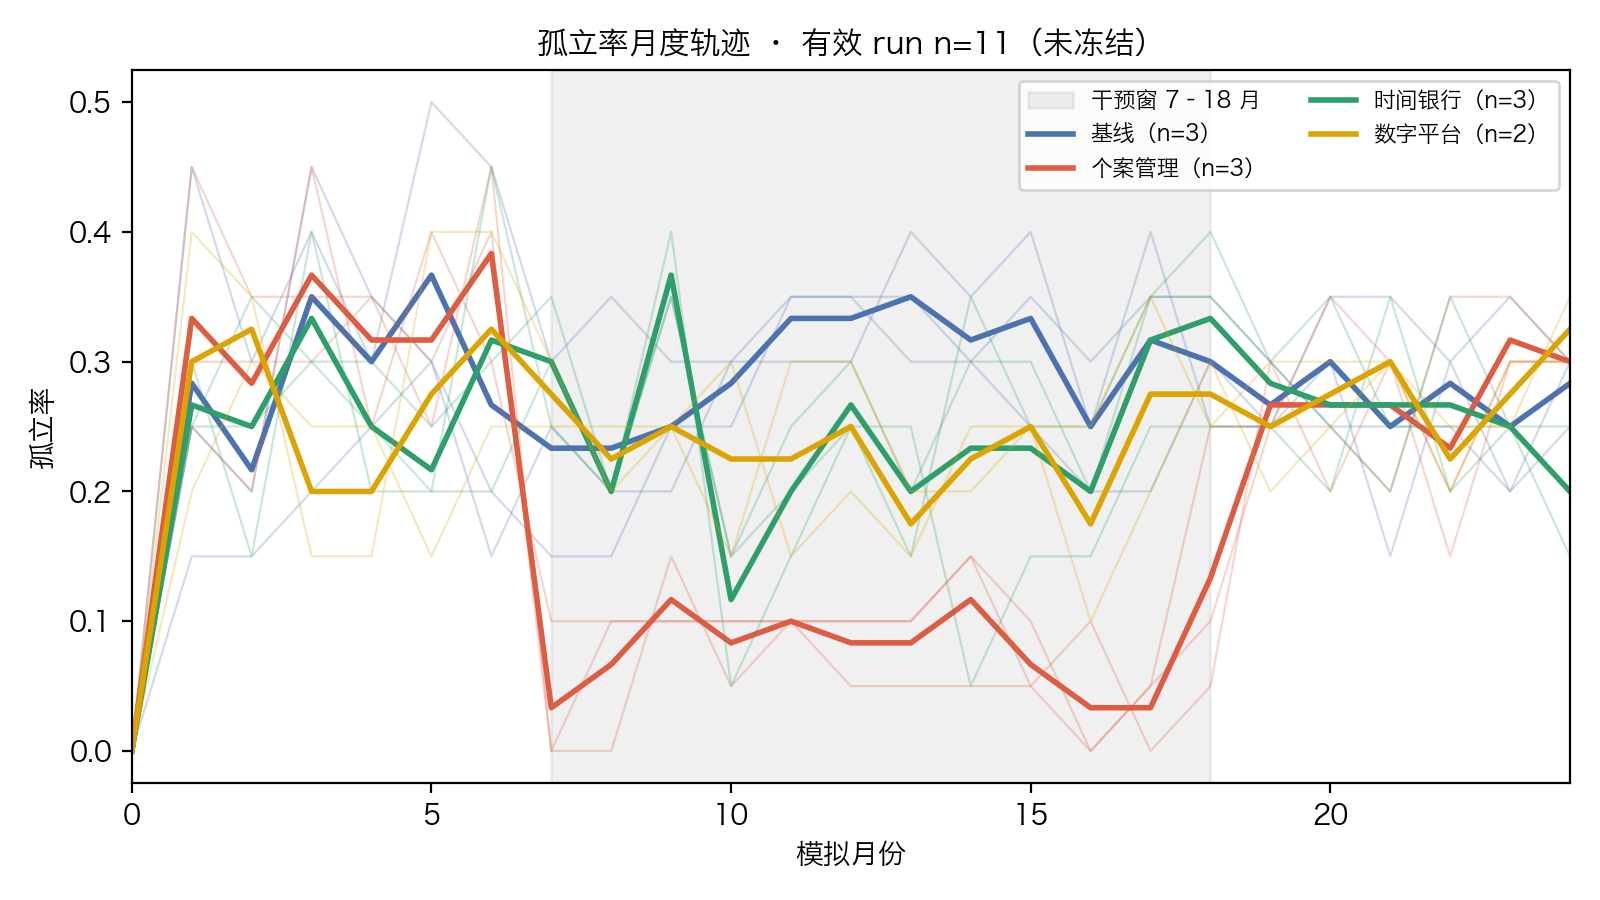
\includegraphics[width=0.95\textwidth]{fig1_trajectory_isolation.png}
\caption{孤立率月度轨迹（粗线为条件均值，细线为单种子，阴影为干预窗第 7--18 月）。个案管理在窗内显著压低孤立率、撤出后迅速回弹的形态清晰可见。}
\label{fig:traj}
\end{figure*}

\subsection{干预期：个案管理领先}
干预期个案管理孤立率 \IsoIvCasework\%，对基线 \IsoIvNone\% 相对下降 \CaseworkIvReduction；同 seed 配对差 \PairIvCasework pp（配对 $n=$\PairIvCaseworkN）。时间银行（\IsoIvTimebank\%）与平台（\IsoIvPlatform\%）改善有限。孤独感（次结局）方向一致：个案管理 \LonIvCasework\% 对基线 \LonIvNone\%。这与 Masi 荟萃中认知类干预效应最大的结论方向一致\citep{masi2011meta}，支持 H1/H2。

\subsection{H4：撤出后的可持续性分化}
撤出后个案管理孤立率反弹 \IsoRebCasework pp（同 seed 配对差 \PairRebCasework pp），干预期优势几乎清零、逼近基线；时间银行反弹 \IsoRebTimebank pp，几乎不反弹（图~\ref{fig:traj}、图~\ref{fig:paired}）。同一机制在规则层独立成立（casework 反弹 \RulesRebCwLo\ 至 \RulesRebCwHi pp、timebank \RulesRebTb pp，20 种子）——\textbf{``结构性互助比外部投入更可持续''在两层模拟中互证}，是本文最有政策价值的发现。机制解释：撤出的是社工这一活跃节点的主动激活，而时间银行结对本身是老人之间的真实关系，部分在撤出后延续。

\begin{figure}[t]
\centering
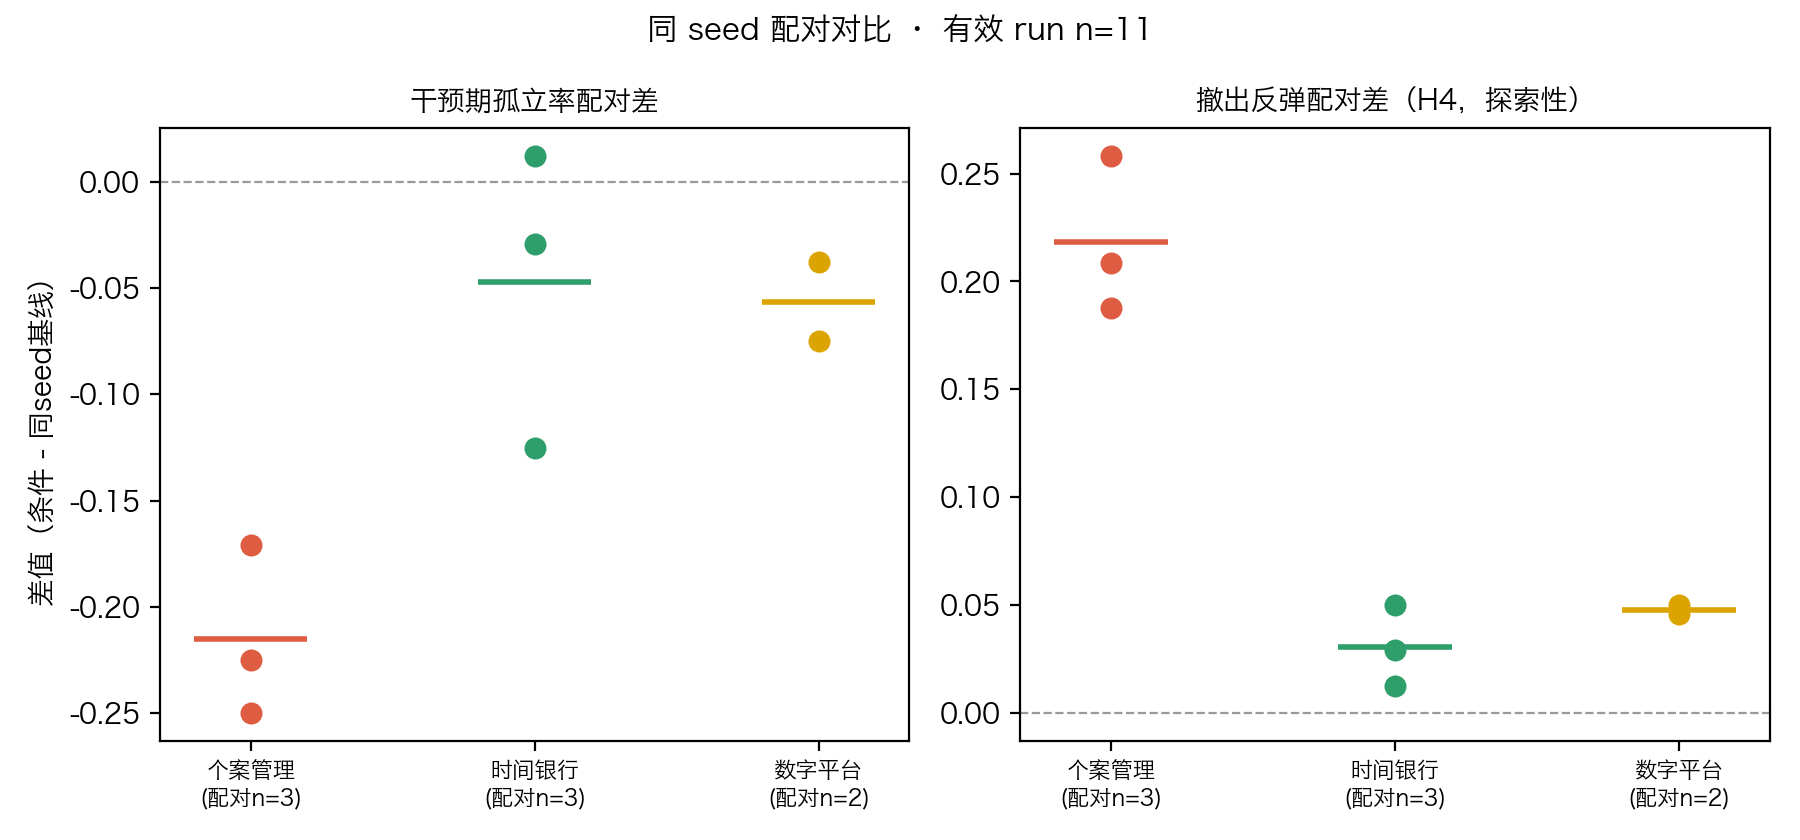
\includegraphics[width=\columnwidth]{fig4_paired_rebound.png}
\caption{同 seed 配对对比（左：干预期效果；右：撤出反弹，探索性）。}
\label{fig:paired}
\end{figure}

\subsection{行为签名与机制佐证（H3）}
三种干预在焦点老人的行为日志中签名清晰可辨\footnote{\ValidRuns\ 个有效 run 的求助请求统计（\texttt{tests/behavior\_signature.json}）：none 3 run 共 249 次、成功 183（73.5\%，均 83.0 次/run）；timebank 247/185（74.9\%，82.3）；casework 412/271（65.8\%，137.3）；platform 2 run 159/94（59.1\%，79.5）。}：时间银行组求助成功率全场最高（结对互助起效）；个案管理组求助请求量最大（社工主动触达）但成功率最低之一；基线组与时间银行组请求量相近，平台组均请求量最少且成功率最低。值得注意的是\textbf{个案管理的``关系数悖论''}：撤出后焦点老人的活跃关系数仍高，但孤立率照样反弹——关系``存在''不等于``起作用''，被撤走的是激活这些关系的社工节点。

个体轨迹把该悖论具体化（预注册选例规则：有效 casework run 中撤出前接受过社工探访、且撤出后孤独感反弹最大的焦点老人；探索性证据）。\CaseCwRun\ 的 \CaseCwAgent\ 号老人在撤出时点（第 18 月）孤独感仅 \CaseCwLonWd、活跃关系 \CaseCwTiesWd\ 条；至第 24 月关系仅减一条（\CaseCwTiesEnd\ 条），孤独感却升至 \CaseCwLonEnd——网络规模几乎未动，失去的只是激活它的社工节点。时间银行侧无来自有效 run 的对应个案（唯一带显式结对记录的 run 未过静默门槛，个案不入证据），如实说明。这对社工实务的含义是：个案管理应内置向互惠型网络的转介与退出计划。

\subsection{两层分歧的如实报告}
干预期排序在两层不完全一致：规则层 timebank 优于 platform，LLM 层 platform 略优于 timebank（平台仅 \NPlatform\ 个有效 seed，该差异无法与种子噪声区分）。机制上可解释：LLM 层的平台干预引入了新志愿者关系、提升活跃关系数。我们将其作为``两层差异及其解释''报告而非掩盖——分层设计的价值恰恰在于暴露这类跨层不一致。

\section{机制层扩展：时机、剂量与自主闭环}\label{sec:mechanism}
\subsection{介入时机的延迟成本}
预注册规则层扫描（启动月 $\{3,5,7,9,12\}\times$ 时长 $\{6,12,18\}\times$ 3 条件，\TimingSeeds\ 种子；基线全时程孤立率 \RulesBaselineOverall\%）得到三点发现：
\begin{enumerate}
  \item \textbf{干预即时起效}：干预期内孤立率几乎不随启动时机变化——延迟的全部代价来自未被保护的等待月份，而非``错过关键窗口''；
  \item \textbf{延迟成本可量化}：启动每推迟一月，两年平均孤立率上升约 \DelayCostCasework pp（casework）/ \DelayCostTimebank pp（timebank）；platform 总效应弱故时机不敏感（\DelayCostPlatform pp）；
  \item \textbf{反弹与剂量无关}：casework 时长从 6 月增至 12 月，撤出反弹不缓解（\RulesRebCwLo\ 至 \RulesRebCwHi pp）——依赖型支持的反弹是机制属性而非剂量不足。
\end{enumerate}
注意披露：晚启动意味着更短的撤出观察窗（混淆），时长 18 月无撤出窗；规则层绝对水平不与 LLM 批次比较，仅取方向与量级。预防期/预警期/危机期的 LLM 行为层时机对照未完成，属后续工作，此处不将计划写作结果。

\subsection{Harness 自主实验闭环}
我们演示了受预注册约束的自动化科研回路：LLM 设计师在预注册搜索空间（条件 $\times$ 启动月 3--12 $\times$ 时长 6--12，目标最小化全时程孤立率，资源帽时长 $\le$12）内逐轮提出候选配置，确定性规则层评估器执行并返回结果，全部 \LoopIters\ 轮审计日志落盘。闭环收敛到 \LoopBestDesc（全时程孤立率 \LoopBestScore\%），与网格最优差异在种子标准差之内——\textbf{闭环流程成立，且我们如实报告它复现了网格平台区、并无超越网格的新发现}。护栏设计（LLM 仅提案、评估确定性、空间与轮数预注册、全轮次落盘）保证该演示不引入选择性报告。此外，逐 run 的自动分析--反思机制（analyze.py）目前实现``发现并标记''，修改实验配置前需人工审核，避免中途改变实验设计。

\section{科学性核查与诚实偏差报告}\label{sec:honest}
\subsection{校准对齐与涌现效度}
输入分布逐维对齐调查数据（第 3.4 节）。运行层动态与文献互证：模拟丧偶冲击方向与 CLHLS 丧偶--孤独动态（丧偶头几年 OR 3.09）一致\citep{yang2021widowhood}。我们只规定画像分布、干预规则与衰减机制；孤立的分布、孤独感轨迹与撤出后互助存续均为涌现结果。

\subsection{关系衰减的结构性限制}
以 Burt 口径实测本模型关系存活曲线（规则层 50 人 $\times$ 48 月）发现两点\textbf{机制层限制}：（1）模型关系流失显著慢于文献（4 年存活 78.8\% 对 Burt 拟合 38.3\%）；（2）存在约 46\% 的存活率地板——有固定联系频率的子女与高频邻里每月刷新联系时间，永不进入衰减分支，因此任何 $\delta$ 取值都无法复现 Burt 幂函数的持续下降。我们据此\textbf{不将关系流失速率作为标定目标}，仅作敏感性维度。引用 Burt 时另有一处更正：其``家庭以外关系半衰期 2.63 年''为原文漏减常数项的算术错误，依原文方程重算应为 1.63 年\citep{burt2000decay}。深度孤立测度受存活率地板截断，故仅入敏感性分析。

\subsection{建模选择的扫描化处理}
三轮独立文献检索（第三轮经多源聚合接口覆盖 CrossRef/OpenAlex/arXiv）一致确认：不存在支持 $\delta=0.06$ 或 caseload $=8$ 的权威文献——凑出``完美吻合''数字的检索结果（本项目在第一轮检索中确曾遇到编造文献与编造数字各一例）已全部否决存档。因此这两个参数按\textbf{建模选择}处理：$\delta$ 扫描 0.06/0.15/0.25（扫描点依实测存活曲线选取）；caseload 在本模型中实际控制高危老人干预覆盖率（4/8/12 对应 40\%/80\%/100\%），与现实登记个案量单位不同——纽约市居家老人个案管理的实测平均登记个案量约 75 人/社工且被认为已超载\citep{pardasani2018caseload}，中国行业标准仅规定人力配置比而无个案量条款\citep{mzt064}，NASW 明确拒绝统一个案量标准\citep{nasw2013}，故按覆盖率维度扫描。扫描结论：$\delta$ 抬升整体水平但不改变干预排序；caseload 干预期内单调、撤出后收敛——覆盖率只影响在场效应，不影响可持续性。

\subsection{失效 run 的根因诊断}
按效度门槛（第~\ref{sec:prereg}~节）判无效的 run 全部归档并逐一诊断，识别出两类失效模式：（1）\textbf{基础设施型}——LLM 网关错误风暴导致整月决策黑洞（错误在 trace 中成簇可见），处置为重跑并调高重试次数（基础设施参数，非协议变更）；（2）\textbf{行为型}——LLM 正常思考但不发起环境行动，集中于干预窗内，与个案依赖机制一致；此类无基础设施可修，按预注册门槛重跑，若复现则按规则排除并在限制节报告门槛张力（门槛可能混同``故障静默''与``依赖性合法不行动''），另做包含该 run 的敏感性分析，不改门槛。

\subsection{模型与推理设定披露}
正式批次使用单一模型（gpt-5.6-sol）与统一采样设置；思考强度未被运行脚本记录，如实标注``未记录''，后续以小样本对照补充。跨模型稳健性（gpt-6-astra 对照批次，seed~1 的 none 与 casework 两条 run）列为敏感性检验，不在主结果内，结果见第~\ref{sec:robust}~节。

\subsection{跨模型敏感性检验}\label{sec:robust}
以 gpt-6-astra 替换焦点老人的驱动模型，其余配置（画像、种子、干预参数、步数）与主批次 seed~1 完全一致，重跑 none 与 casework 两条 run，比较 casework$-$none 的干预期孤立率差与撤出反弹方向是否与主模型一致。单 seed、双条件，仅作描述性方向判断，不做显著性声称。结果与静默率对照见表~\ref{tab:robust}。

\textbf{方向一致。}两模型下 casework 相对 none 均呈``干预期压低 $+$ 撤出后反弹更大''：主模型配对差为干预期 $-17.1$~pp、反弹 $+18.8$~pp；gpt-6-astra 为干预期 $-25.0$~pp、反弹 $+25.0$~pp，且撤出期两臂孤立率回到同一水平（均为 30.0\%），即 casework 的效果在撤出后完全消失，与前文``注入型节点''解释一致。

\textbf{行为型静默是模型特征而非偶然故障。}gpt-6-astra 的 none 臂两次独立运行（同一 seed）静默率分别为 10.7\%（16/150 agent-月）与 11.3\%（17/150），均越过 10\% 效度门槛并按规则判无效；两次运行的 LLM 错误率分别为 0.17\% 与 0，静默分散在多位老人的多个月份而非集中于网关超时步，与 platform seed~2 的基础设施型失效不同。主批次 11 条 sol run 静默率全部 $\le 10\%$（none seed~1 为 4.0\%），而同一模型的 casework 臂静默率仅 2.0\%——外部行动者持续来访似乎``拉动''了 astra 焦点老人产出决策，无人干预时该模型更倾向于不给出任何行动。我们将此本身作为稳健性发现报告：（i）门槛按主模型设定，对更``沉默''的模型可能系统性偏严，局限节对此作出说明；（ii）表中 astra none 臂的孤立率仅供方向参考，不进入任何主结果；（iii）第三次重跑被明确放弃，以避免``跑到通过为止''的选择性报告。

\begin{table}[t]
\centering\small
\caption{跨模型敏感性检验（seed~1，单 run）。孤立率为窗口均值（\%），反弹 $=$ 撤出期 $-$ 干预期（pp）；静默率为焦点老人无决策 agent-月占比（门槛 10\%）。}
\label{tab:robust}
\begin{tabular}{llcccc}
\toprule
模型 & 条件 & 静默率 & 干预期 & 撤出期 & 反弹 \\
\midrule
gpt-5.6-sol & none     & 4.0\% & 25.8 & 25.0 & $-0.8$ \\
            & casework & 8.7\% & 8.8  & 26.7 & $+17.9$ \\
gpt-6-astra & none     & 11.3\%$^\dagger$ & 29.6 & 30.0 & $+0.4$ \\
            & casework & 2.0\% & 4.6  & 30.0 & $+25.4$ \\
\midrule
\multicolumn{2}{l}{配对差 casework$-$none：sol}   & & $-17.1$ & $+1.7$ & $+18.8$ \\
\multicolumn{2}{l}{配对差 casework$-$none：astra} & & $-25.0$ & $0.0$ & $+25.0$ \\
\bottomrule
\end{tabular}

\smallskip
{\footnotesize $^\dagger$ 超过 10\% 门槛判无效；首次运行为 10.7\%（16/150），同样越线，行为指标仅供方向参考。}
\end{table}

\section{真实成本核算}
多智能体 LLM 实验的成本报告必须计入被质量门槛淘汰的 run。本项目累计 LLM 调用 \TotalCalls\ 次（trace 实测，含归档失效 run），估算总成本 \$\CostTotal：主批次有效 run \$\CostValid、无效沉没 \$\CostWasted（占主批次 \WasteShare），另有跨模型对比臂 \$\CostModelCompare（第~\ref{sec:robust}~节）。token 用量为文档化假设（trace 未记录逐调用用量）、单价按公开定价，口径随数据文件公开。分层设计的意义在此具体化：规则层扫描（\TimingSeeds\ 种子 $\times$ 45 配置）与 harness 闭环全部零 API 成本；若以 LLM 层完成同等扫描，成本将超出主批次一个数量级。

\section{讨论与政策含义}
\textbf{（一）轮候时间本身是干预设计变量。}机制层估计表明干预即时起效、延迟成本按月线性累积（约 \DelayCostCasework pp/月）。对实务的含义：压缩从识别到开案的行政周期，其收益与提高干预强度同阶。

\textbf{（二）个案管理需要内置退出计划。}干预期效果最强与撤出后反弹最大是同一机制的两面：社工是被注入的活跃节点。反弹不随剂量缓解，提示退出设计（逐步减量、向互惠网络转介）应作为个案管理的标准组件而非可选项——这与``关系数悖论''（关系仍在、激活已失）的行为证据一致。

\textbf{（三）结构性互助的政策价值在撤出之后。}时间银行干预期效果不及个案管理，但其建立的对等关系在撤出后延续。若政策目标是长期可持续性而非短期指标，两类干预的组合（个案管理开路、时间银行接续）值得作为后续实验方向。

\textbf{（四）弱干预谈时机无意义。}平台类干预总效应弱，时机不敏感——先保证强度，再优化时机。

以上均为模型机制结论，用于生成可检验的政策假设，\textbf{不宣称真实人群的因果效应}。

\section{局限与伦理}
\textbf{局限。}（1）$n=3$ 种子（平台臂 $n=\NPlatform$）只支持描述性对比与方向判断，不支持显著性与稳定排序；（2）关系衰减机制存在 46\% 存活率地板，慢于文献实证形态；（3）LLM 焦点老人的行为效度依赖模型本身，行为型静默与真实老人的``合法不行动''难以区分，且 10\% 静默门槛按主模型 gpt-5.6-sol 设定，对更倾向``不行动''的模型（gpt-6-astra none 臂两次为 10.7--11.3\%）可能系统性偏严，见第~\ref{sec:robust}~节；（4）校准数据存在口径差（调查波次、独居子样本 vs 全体）；（5）撤出观察窗仅 6 个月；（6）Ristolainen RCT 的亚组效应存在基线不可比问题\citep{ristolainen2020effects}，个案管理参数依据以 Masi 荟萃为主。

\textbf{伦理。}全部智能体为模拟实体，不涉及真实个人；调查数据仅使用公开微观数据的聚合分布；LLM 生成的``老人理由''是机制探针而非真实老人话语，论文避免将其拟人化引用。模拟结论若被直接当作资源分配依据存在误用风险，故本文反复强调其假设生成属性。

\section{结论}
本文以分层混合生成式智能体模拟回答了传统数据无法回答的两个问题：干预撤出之后（个案管理反弹、时间银行延续，两层互证）与何时介入（即时起效、延迟成本按月累积）。方法论上，我们提供了一套可迁移的科学性纪律：预注册与效度门槛、真实数据锚定与偏差如实报告、失效根因诊断、含沉没成本的成本透明、以及受护栏约束的自主实验闭环。批次冻结后全部数字经脚本自动更新，欢迎按附录复现。

\bibliographystyle{unsrtnat}
\bibliography{refs}

\appendix
\section{可复现性清单}\label{app:repro}
\begin{itemize}
  \raggedright % 清单多为不可断行的等宽路径，两端对齐会把行内空白拉得过大
  \item \textbf{代码与数据}：AgentSociety2 仓库 \texttt{examples/v2/elder\_support/}；环境模块 \texttt{custom/envs/elder\_support\_env.py}。
  \item \textbf{正式批次}：\texttt{run\_batch.sh 24 1 2 3}（断点自动续跑；效度门槛与归档逻辑内置）。
  \item \textbf{分析与图表}：\texttt{tools/compare\_conditions.py} $\rightarrow$ \texttt{comparison.json}；\texttt{tools/make\_figures.py}（每图配同名 CSV）；\texttt{tools/gen\_paper\_numbers.py}（本文全部数字的唯一来源）。
  \item \textbf{机制扫描与闭环}：\texttt{tests/scan\_timing.py}、\texttt{tools/harness\_loop.py}（预注册头部 + 逐轮 JSONL 审计日志）。
  \item \textbf{成本与诊断}：\texttt{tools/cost\_report.py}、\texttt{tests/silence\_diagnosis.json}。
  \item \textbf{校准文档}：\texttt{data\_pipeline/out/} 下 \texttt{calibration\_targets.md} 与 \texttt{references\_verified.md}（含已否决条目与核实方法）。
  \item \textbf{实时面板}：\url{https://agentsociety.shangdian.me}（批次进度、结论卡片、机制证据、成本与失效诊断）。
\end{itemize}

\section{效度门槛判定细则}
run 有效当且仅当：DONE 标志存在；月度指标 0--24 完整；决策记录非空；6 名焦点老人合计静默率 $\le$10\%（严格大于 0.10 判无效）；LLM 调用错误率 $\le$5\%。判无效的 run 以时间戳目录归档（\texttt{*.invalid-<timestamp>}），保留全部 trace 与决策日志供诊断，不删除。

\end{document}
